\documentclass[
	% -- opções da classe memoir --
	12pt,				% tamanho da fonte
	openright,			% capítulos começam em pág ímpar (insere página vazia caso preciso)
	oneside,			% para impressão em frente e verso. Oposto a oneside
	a4paper,			% tamanho do papel.
	% -- opções da classe abntex2 --
	chapter=TITLE,		% títulos de capítulos convertidos em letras maiúsculas
	%section=TITLE,		% títulos de seções convertidos em letras maiúsculas
	%subsection=TITLE,	% títulos de subseções convertidos em letras maiúsculas
	%subsubsection=TITLE,% títulos de subsubseções convertidos em letras maiúsculas
	% -- opções do pacote babel --
	english,			% idioma adicional para hifenização
	french,				% idioma adicional para hifenização
	spanish,			% idioma adicional para hifenização
	brazil				% o último idioma é o principal do documento
	]{abntex2}
% ---
% Pacotes básicos 
% ---
\usepackage{lmodern}			% Usa a fonte Latin Modern
\usepackage{mathptmx}			% Usa a fonte Times New Roman
\usepackage[T1]{fontenc}		% Selecao de codigos de fonte.
\usepackage[utf8]{inputenc}		% Codificacao do documento (conversão automática dos acentos)
\usepackage{lastpage}			% Usado pela Ficha catalográfica
\usepackage{indentfirst}		% Indenta o primeiro parágrafo de cada seção.
\usepackage{color}				% Controle das cores
\usepackage{graphicx}			% Inclusão de gráficos
\usepackage{subcaption}				% Inclusão de gráficos lado a lado
\usepackage{microtype} 			% para melhorias de justificação
\usepackage{tabularx,ragged2e}	% Para inserir tabelas
\usepackage{multirow}			% Para mesclar células
\usepackage[dvipsnames,table,xcdraw]{xcolor}		% Permite adicionar cores nas linhas de tabelas
\usepackage{fancyvrb}			% Permite adicionar arquivos de texto
\usepackage[portuguese, ruled, linesnumbered]{algorithm2e} % Uso de algoritmos
\usepackage{amsfonts}			% Permite usar notação de conjuntos
\usepackage{amsmath}			% Permite citar equações
\usepackage{amsthm}				% Permite criar teoremas e experimentos
\usepackage[font={bf, small}, labelsep=endash, labelfont=bf]{caption}	% Faz legenda de figuras ficarem em negrito
\usepackage{cancel}				% Permite fazer expressão tendendo a zero
\usepackage{epstopdf}			% Converte eps para pdf
\usepackage[final]{pdfpages}
\usepackage{hyperref}
\usepackage{fancybox}


\newcolumntype{L}{>{\RaggedRight\arraybackslash}X}
% ---
% ---
% Pacotes adicionais, usados apenas no âmbito do Modelo Canônico do abnteX2
% ---
\usepackage{lipsum}				% para geração de dummy text
% ---
% ---
% Pacotes de citações
% ---
%\usepackage[brazilian,hyperpageref]{backref}	 % Paginas com as citações na bibl
\usepackage[alf, abnt-emphasize=bf]{abntex2cite}	% Citações padrão ABNT
% ---
% Customizações para o layout da UFPA
% ---
\usepackage{modelo-ufpa/ufpa}
% Muda o título de lista de ilustrações para lista de figuras
\addto\captionsbrazil{%
  \renewcommand{\listfigurename}%
    {Lista de Ilustrações}%
	\renewcommand{\listtablename}%
    {Lista de Tabelas}%
}
% Permite utilizar figuras sem precisar colocar o caminho absoluto
\graphicspath{{imagens/}}
% Define o ambiente de experimentos
\theoremstyle{definition}
\newtheorem{experimento}{Experimento}[section]
\newcommand{\experimentoautorefname}{Experimento}


% --------------------------------------------------------------
% Informações do TRABALHO
% --------------------------------------------------------------
\universidade{UNIVERSIDADE FEDERAL DO PARÁ}
\instituto{INSTITUTO DE TECNOLOGIA}
\faculdade{FACULDADE DE COMPUTAÇÃO E TELECOMUNICAÇÕES}
%\curso{CURSO DE BACHARELADO EM SISTEMAS DE INFORMAÇÃO}
\titulo{RELATÓRIO DE SO}
\autor{
%\begin{tabular}{l l}
    DAVID PINHEIRO DE SOUSA - 202207040045 \\
    JOAO VICTOR SANTOS BRITO FERREIRA - 202207040028 \\
    JOEL TAVARES MIRANDA - 202206840054 \\
    KAUAN MIRANDA TAVARES - 202206840033 \\
    MARCO ANTONIO DO ESPIRITO SANTO MAUES JUNIOR - 202206840038 \\
%\end{tabular}
}
\local{Belém}
\data{2023}
\orientador{Prof. Dr. Diego Lisboa Cardoso}
\tipotrabalho{Monografia}

% o nome da instituição e a área de concentração 
\preambulo{Relatório do trabalho 2 de Sistemas Operacionais.}
%\sobrenome{Sobrenome}
%\nome{Nome}
%\palavraschave
%\datadadefesa{Data da Defesa: 09 de Março de 2017}%07 de Dezembro de 2016}
\conceito{Conceito: Excelente}
\faculdadedoorientador{Faculdade de Computação e Telecomunicações - UFPA}
%\primeiromembrodabanca{Prof. Dr. Nome Sobrenome}
%\faculdadedoprimeiromembrodabanca{}
%\segundomembrodabanca{}
%\faculdadedosegundomembrodabanca{}
% -------------------------------------------------------------------------
% ---
% Configurações de aparência do PDF final
% alterando o aspecto da cor azul
\definecolor{blue}{RGB}{41,5,195}
% informações do PDF
\makeatletter
\hypersetup{
     	%pagebackref=true,
		pdftitle={\imprimirtitulo}, 
		pdfauthor={\imprimirautor},
    	pdfsubject={\imprimirpreambulo},
	    pdfcreator={LaTeX with abnTeX2},
		pdfkeywords={\imprimirpalavraschave}, 
		colorlinks=true,       		% false: boxed links; true: colored links
    	linkcolor=black,          	% color of internal links
    	citecolor=black,        		% color of links to bibliography
    	filecolor=magenta,      		% color of file links
		urlcolor=blue,
		bookmarksdepth=4,
        breaklinks=true
}
\makeatother
% --- 
% Espaçamentos entre linhas e parágrafos 
% --- 
% O tamanho do parágrafo é dado por:
\setlength{\parindent}{1.3cm}
% Controle do espaçamento entre um parágrafo e outro:
\setlength{\parskip}{0.2cm}  % tente também \onelineskip
% compila o indice
% ---
\makeindex
% ---

% -------------------------------------------------------------------------
% ---------------------------INICIO DO DOCUMENTO---------------------------
% -------------------------------------------------------------------------
\begin{document}
% Seleciona o idioma do documento (conforme pacotes do babel)
\selectlanguage{brazil}
% Retira espaço extra obsoleto entre as frases.
\frenchspacing 
% ----------------------------------------------------------
% ELEMENTOS PRÉ-TEXTUAIS
% ----------------------------------------------------------
% \pretextual

% ---
% Capa
% ---
\imprimircapa
% ---

% ---
% Folha de rosto

\imprimirfolhaderosto

\newpage

\setlength{\absparsep}{18pt} % ajusta o espaçamento dos parágrafos do resumo

\pdfbookmark[0]{\contentsname}{toc}
\tableofcontents*
\cleardoublepage
% ---
% ---------------------------------------------------------
% ELEMENTOS TEXTUAIS
% ----------------------------------------------------------
\textual

% ----------------------------------------------------------
% Introdução
% ----------------------------------------------------------

\chapter{Introdução}

Este trabalho aborda a implementação de concorrência e 
sincronismo por meio da criação de processos e threads. O 
trabalho consiste em uma série de tarefas que exploram diferentes 
aspectos da criação de processos, comunicação entre processos e o 
uso de threads em um ambiente Linux. Através dessas atividades, 
pretendemos aprofundar nossa compreensão de como a concorrência é 
gerenciada em sistemas operacionais e como diferentes abordagens afetam 
o desempenho e o comportamento do programa.


\chapter{Objetivos}

O principal propósito deste trabalho é:

\begin{itemize}
    \item \textbf{Criação de Processos}:
    \begin{itemize}
        \item Implementar a criação de processos de acordo com as hierarquias e requisitos especificados, incluindo cenários com avô, pai e filho, bem como múltiplos filhos.
    \end{itemize}

    \item \textbf{Comunicação entre Processos e Threads}:
    \begin{itemize}
        \item Explorar a comunicação entre processos e threads, incluindo o compartilhamento de variáveis e recursos entre eles.
    \end{itemize}

    \item \textbf{Comparação de Desempenho}:
    \begin{itemize}
        \item Comparar o desempenho da criação de processos e threads para realizar as tarefas do programa. Calcular a média de tempo de 20 simulações para obter uma análise precisa.
    \end{itemize}

    \item \textbf{Teste de Limites Máximos}:
    \begin{itemize}
        \item Testar e identificar os limites máximos da quantidade de processos e threads que podem ser disparados em um ambiente Linux. Explorar as configurações relacionadas.
    \end{itemize}
\end{itemize}

  

\chapter{Desenvolvimento (Programa explicado e Cópias das telas do emulador.)}

Primeiramente, o desenvolvimento deste trabalho gira em torno da criação
de processos, que é uma parte fundamental dos sistemas operacionais. 
Os sistemas operacionais permitem que programas criem novos processos, que 
podem ser vistos como tarefas independentes que compartilham recursos do sistema. 

A criação de processos deste trabalho é baseada nos requisitos e níveis de hierarquia descritos 
no roteiro e evidenciados nas seções deste capítulo.

%\begin{enumerate}
%    \item 
%   \item
%    \item Programa com 1 Avô, 1 Pai e 1 Filho, "elimine" o processo 'Pai' e veja quem será o novo pai do processo 'Filho'.
%   \item Programa que cria 3 threads. A primeira escreve na tela “A”, a segunda “B” e a terceira “C”. Faça que seja sempre escrito na tela “ABC”.
%    \item Para o processo Pai e filho, declare uma variável visível ao pai e ao filho, no pai inicialize a variável com 1 e imprima seu valor antes do fork(). No filho, altere o valor da variável para 5 e imprima o seu valor antes do exit(). Agora, no pai, imprima novamente o valor da variável após o filho ter alterado a variável - após a waitpid(). Justifique os resultados obtidos.
%    \item Ordenar um vetor de 100 posições em processos e threads. O filho ordena o vetor e o pai exibe os dados do vetor antes da criação do filho (fork) e depois da espera pelo filho (waitpid para processos). Eles usarão o mesmo vetor na memória? Justifique.
%    \item . Os limites máximos. Em ambiente linux os limites superiores da quantidade de processos e threads que podem ser disparados são configuráveis, testar e identificar.
%    \item Programa para comparar o desempenho para a realização da(s) tarefa(s) do programa através do uso de primitivas fork e através de threads (calcule a média de tempo de 20 simulações).
%\end{enumerate}

\section{Programa com 1 Avô, 1 Pai e 1 Filho}


A função \texttt{fork()} em C é comumente usada para criar novos processos. 
A chamada \texttt{fork()} cria uma cópia exata do processo existente, 
resultando em dois processos independentes - o processo pai e o processo filho. 
O processo pai e o processo filho compartilham o mesmo código, mas têm 
seu próprio espaço de endereçamento de memória. Isso é frequentemente usado 
para criar hierarquias de processos, onde um processo pai pode criar um ou 
mais processos filhos.

O código mostrado na figura \ref{fig:processo1} demonstra a criação de uma hierarquia de processos 
com um avô, um pai e um filho (neto) usando a função \texttt{fork()}. 
Aqui está uma descrição detalhada do código:

\begin{figure}
    \centering
    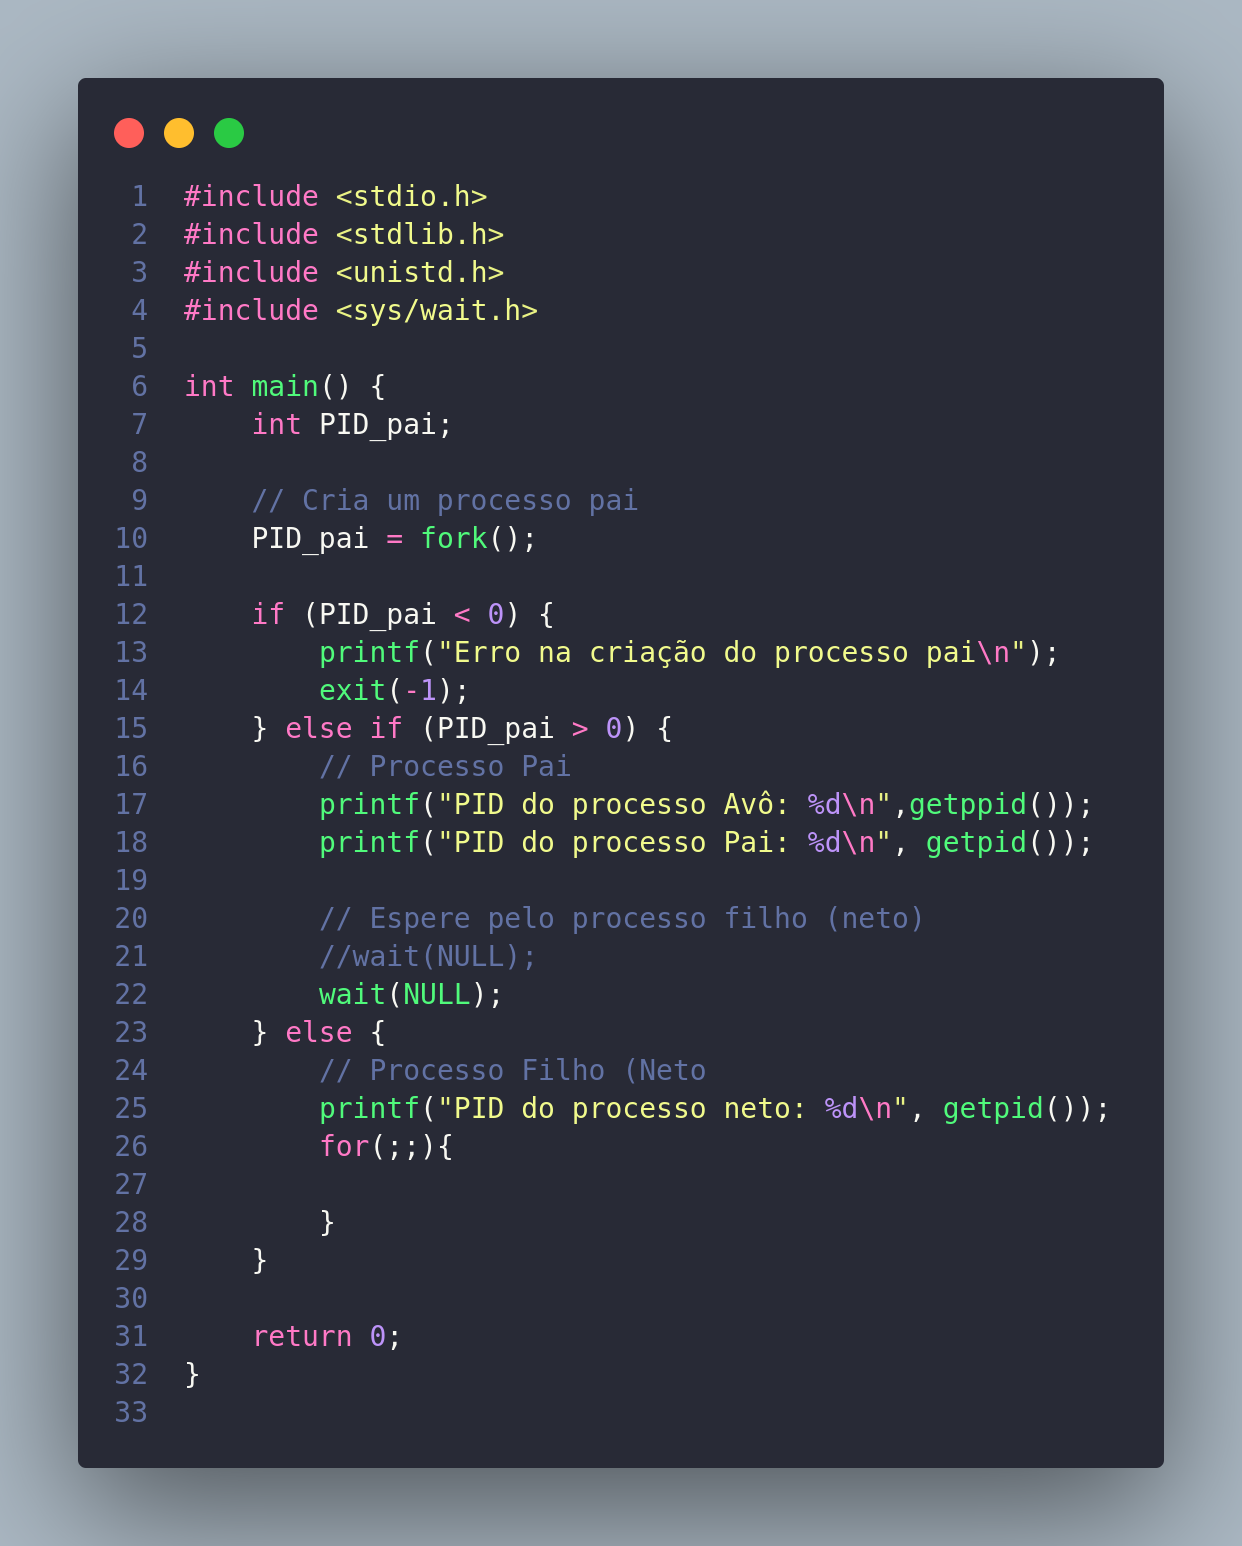
\includegraphics[width=0.5\textwidth]{imagens/processos_1.png}
	\caption{Código em C. Disponível em: \href{https://github.com/jvictorferreira3301/Sistemas_Operacionais/blob/main/2_thread/2-1_processo_avo_pai_filho.c}{github.com/jvictorferreira3301/SistemasOperacionais/blob/main
    /2\_thread/2-1\_processo\_avo\_pai\_filho.c}}
	\label{fig:processo1}
\end{figure}


\begin{itemize}
    \item \texttt{\#include} direciona a inclusão de bibliotecas necessárias, como entrada/saída padrão e manipulação de processos.
    \item A função \texttt{main()} é o ponto de entrada do programa.
    \item \texttt{int PID\_pai} é uma variável inteira que armazenará o PID do processo pai.
    \item \texttt{PID\_pai = fork();} cria um novo processo através da chamada \texttt{fork()} e armazena o valor de retorno em \texttt{PID\_pai}. O processo pai receberá o PID do filho, enquanto o processo filho receberá 0. !!!!corrigir aqui!!!!
    \item O código verifica se \texttt{PID\_pai} é menor que 0, o que indicaria um erro na criação do processo pai, e nesse caso, exibe uma mensagem de erro e encerra o programa.
    \item Se \texttt{PID\_pai} for maior que 0, isso significa que estamos no processo pai. O código exibe o PID do processo avô (obtido com \texttt{getppid()}) e o PID do processo pai (obtido com \texttt{getpid()}). Em seguida, aguarda a conclusão do processo filho (neto) usando \texttt{wait(NULL)}.
    \item Se \texttt{PID\_pai} for igual a 0, isso significa que estamos no processo filho (neto). O código exibe o PID do processo filho (neto) e entra em um loop infinito, mantendo o processo filho em execução.
\end{itemize}

Em suma, esse código cria uma estrutura hierárquica de três processos: avô, 
pai e filho (neto). O processo avô cria o processo pai, 
que por sua vez cria o processo filho. Isso demonstra a 
criação de processos em uma hierarquia usando \texttt{fork()} e é 
um conceito fundamental em sistemas operacionais. Podemos ver 
a execução desse código na figura~\ref{fig:run_processo1} no terminal ZSH do linux

\begin{figure}
    \centering
    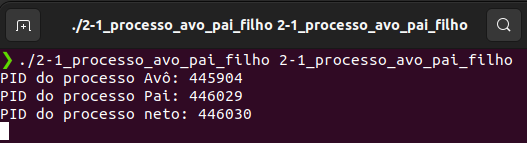
\includegraphics[width=1.0\textwidth]{imagens/run_processos_1.png}
	\caption{Execuçao do código em C. }
	\label{fig:run_processo1}
\end{figure}

\section{Programa com 1 Pai e 2 Filhos}

Nesta seção é mostrado o código em linguagem C, na figura \ref{fig:processos2}, que demonstra a 
criação de um processo pai e dois processos filhos. Essa demonstração ajudará 
a ilustrar o conceito de hierarquia de processos, onde um processo pai pode 
criar e controlar vários processos filhos.

\begin{itemize}
    \item \texttt{\#include} direciona a inclusão de bibliotecas necessárias, como entrada/saída padrão e manipulação de processos.
    \item A função \texttt{main()} é o ponto de entrada do programa, onde a execução começa.
    \item \texttt{int pid\_filho1} é uma variável inteira que será usada para armazenar o PID do primeiro processo filho (Filho 1).
    \item \texttt{pid\_filho1 = fork();} cria um novo processo por meio da chamada da função \texttt{fork()} e armazena o valor de retorno em \texttt{pid\_filho1}. O processo pai receberá o PID do primeiro filho, enquanto o processo filho (Filho 1) receberá 0.
    \item O código verifica se \texttt{pid\_filho1} é menor que 0, o que indicaria um erro na criação do processo filho. Nesse caso, é exibida uma mensagem de erro e o programa é encerrado.
    \item Se \texttt{pid\_filho1} for maior que 0, isso significa que estamos no processo pai. O código exibe o PID do processo pai atual (obtido com \texttt{getpid()}). Em seguida, ele cria o segundo processo filho (Filho 2) usando outra chamada à função \texttt{fork()}, criando assim uma hierarquia de processos. 
    \item Se \texttt{pid\_filho2} for menor que 0, indica um erro na criação do segundo processo filho, e uma mensagem de erro é exibida.
    \item Se \texttt{pid\_filho2} for igual a 0, isso significa que estamos no segundo processo filho (Filho 2). O código exibe o PID do processo filho 2 e o PID de seu pai (processo pai). 
    \item O processo pai, identificado pelo \texttt{else}, aguarda a conclusão do primeiro filho (Filho 1) usando \texttt{wait(NULL)}.
    \item Posteriormente, o processo pai aguarda a conclusão do segundo filho (Filho 2) usando \texttt{wait(NULL)}. Finalmente, o processo pai encerra sua execução.

\end{itemize}

Na figura \ref{fig:run2} é mostrada a execução do código da figura \ref{fig:processos2}
no terminal ZSH do linux. 

\begin{figure}
    \centering
    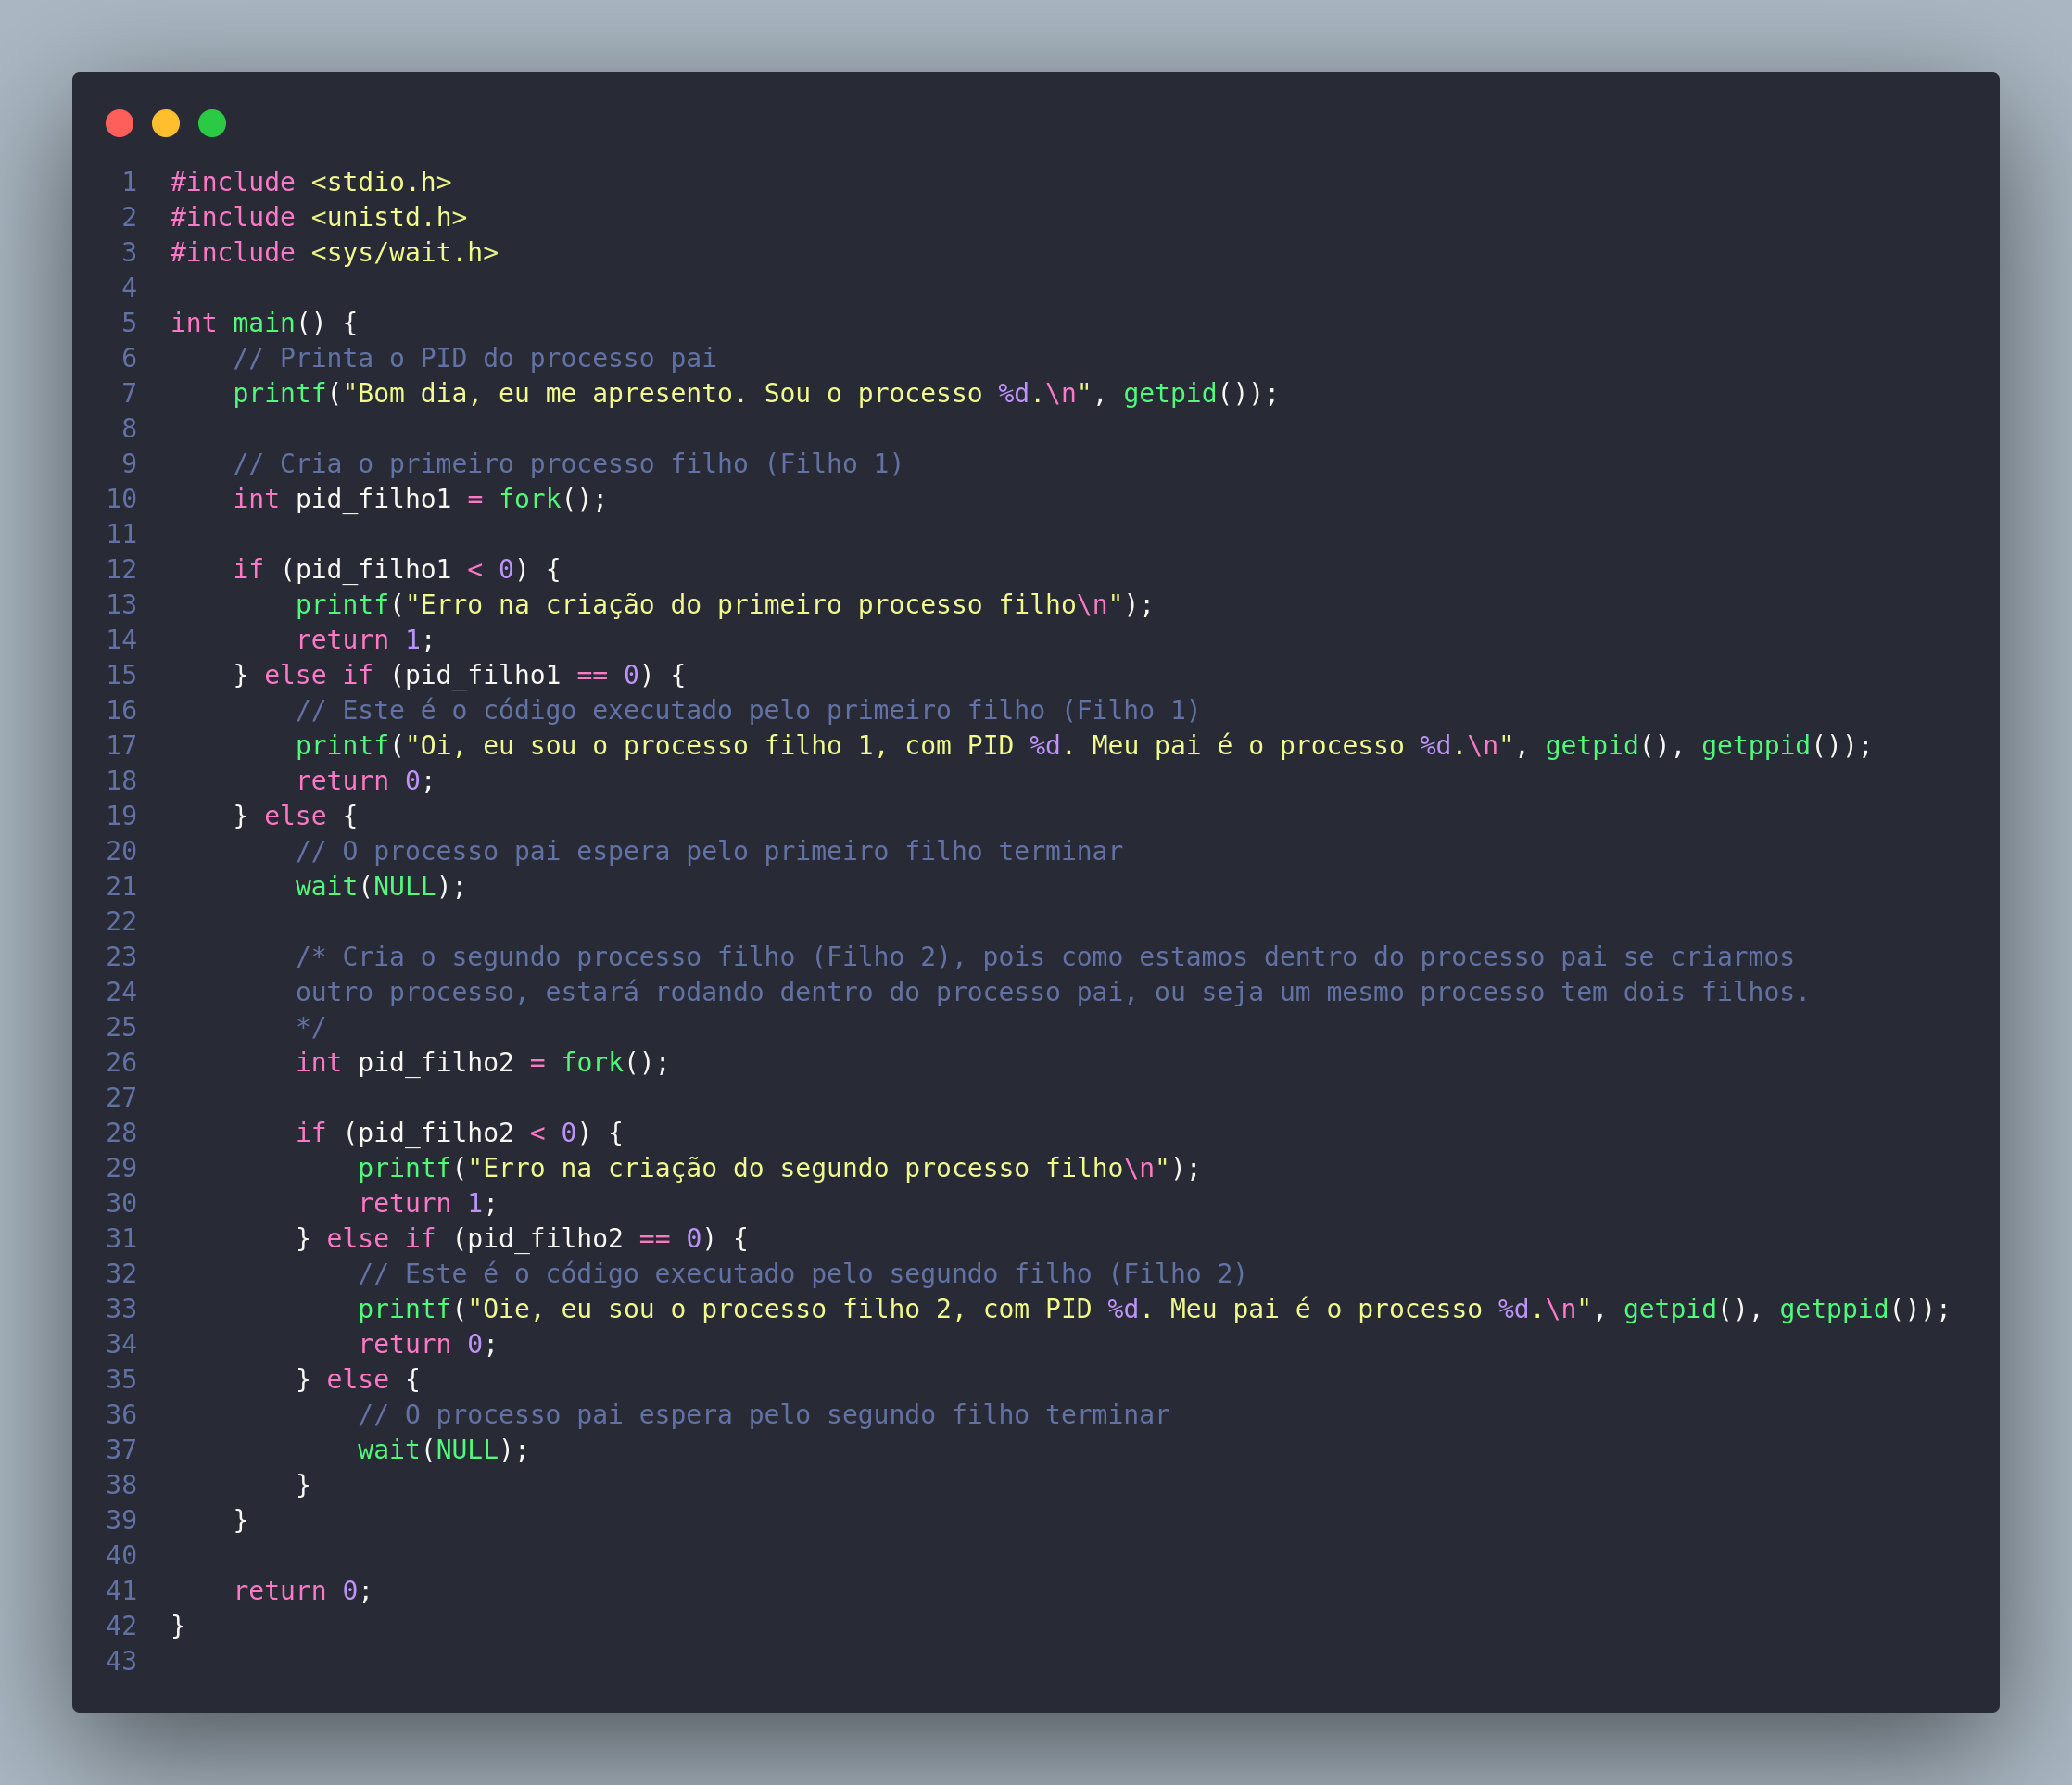
\includegraphics[width=0.7\textwidth]{imagens/processos_2.png}
    \caption{Código em C. Disponível em: \href{https://github.com/jvictorferreira3301/Sistemas_Operacionais/blob/main/2_thread/2-2_processo_pai_2filho.c}{github.com/jvictorferreira3301/SistemasOperacionais/blob/main
    /2\_thread/2-2\_processo\_pai\_2filho.c}}
    \label{fig:processos2}
\end{figure}

\begin{figure}
    \centering
    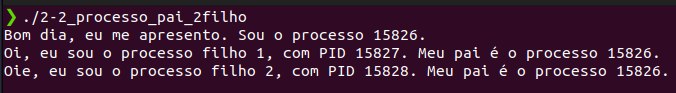
\includegraphics[width=0.7\textwidth]{imagens/run_processos_2.png}
    \caption{Execução do Código em C.}
    \label{fig:run2}
\end{figure}

\section{Programa com 1 Avô, 1 Pai e 1 Filho; Parricídio}

\section{Thread ABC}

Nesta seção, apresentaremos um exemplo prático em C, no qual três threads são 
criadas para imprimir as letras "A", "B" e "C" na tela, garantindo que 
a sequência "ABC" seja sempre exibida. Isso demonstrará como as threads 
podem ser usadas para coordenar tarefas concorrentes e sincronizar a saída.

\begin{itemize}
    \item \texttt{\#include} direciona a inclusão das bibliotecas necessárias, como pthread (para manipulação de threads), entrada/saída padrão e manipulação de processos.
    \item A função \texttt{main()} é o ponto de entrada do programa, onde a execução começa.
    \item \texttt{void *print\_abc(void *threadid)} é a função que cada thread executará. Cada thread recebe um identificador \texttt{threadid} e, com base nesse identificador, decide qual letra imprimir ("A", "B" ou "C") com intervalos de tempo diferentes.
    \item O código utiliza a função \texttt{pthread\_create} para criar três threads, cada uma chamando a função \texttt{print\_abc} com um identificador único.
    \item As threads são projetadas para imprimir as letras com intervalos de tempo específicos (1 segundo, 2 segundos e 3 segundos, respectivamente), criando assim a sequência "ABC".

\end{itemize}

\begin{figure}
    \centering
    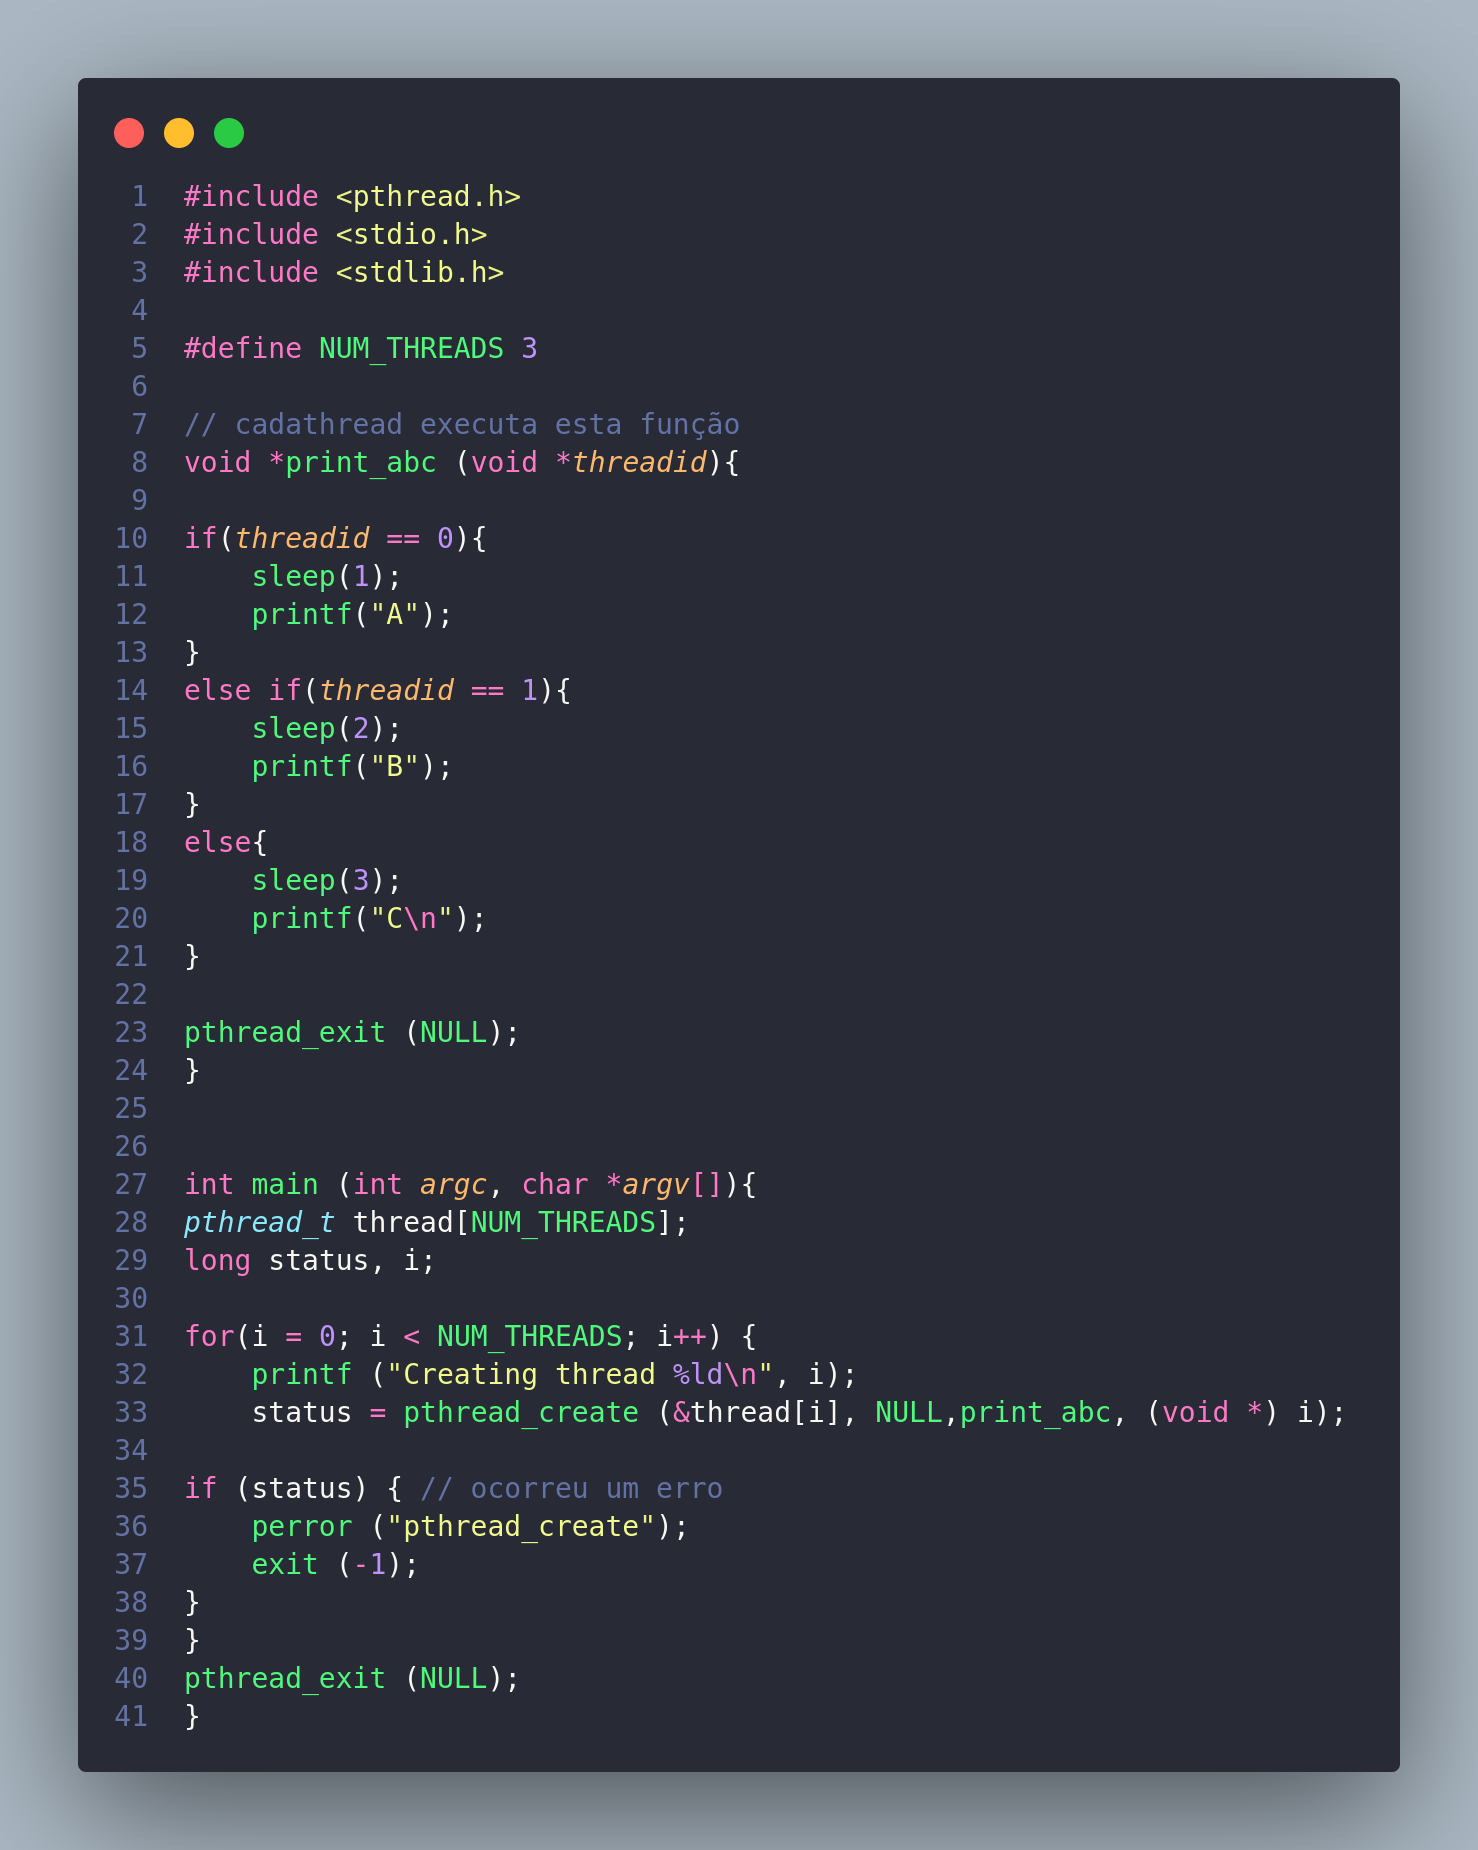
\includegraphics[width=0.6\textwidth]{imagens/processos_4.png}
	\caption{sss.}
	\label{fig:dddd}
\end{figure}

\begin{figure}
    \centering
    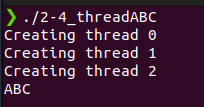
\includegraphics[width=0.6\textwidth]{imagens/run_processos_4.png}
    \caption{.}
    \label{fig:dd}
\end{figure}
\section{Processo Pai e Filho}

\section{Vetor de 100 posições}

\section{Threads versus Processos}

\section{Benchmark}

\chapter{Conclusão}
\label{conclusao}





\postextual

\bibliography{bibliografia}

\cite{tanenbaum2010sistemas}

\end{document}
